\section{Enumeration of vulnerable resources}
\subsection{Global campaign 1}
Input data set: 
\begin{itemize}
 \item 3,277,097,568 domain/server pairs
 \item 327,688,010 unique domains
 \item 3,448,271 unique DNS servers
\end{itemize}

Vulnerable resources:
\begin{itemize}
 \item 579,186(0.018\%) domain/server pairs
 \item 309,687(0.095\%) unique domains
 \item 5738(0.166\%) unique DNS servers
\end{itemize}

\subsection{Global campaign 2}

Input data set: 
\begin{itemize}
 \item 5,032,117,394 domain/server pairs
 \item 353,870,509 unique domains
 \item 3,855,614 unique DNS servers
\end{itemize}

Vulnerable resources:
\begin{itemize}
 \item 679,930(0.014\%) domain/server pairs
 \item 381,965(0.108\%) unique domains
 \item 5576*0.145\%) unique DNS servers
\end{itemize}



\subsection{Short-lived domains}
\subsection{Vulnerable subdomains}
\subsection{Propagation between primary and secondary name servers - Michał}
%\begin{table}[h!]
%\begin{center}
%\caption{Propagation results. \label{tab:propagation}}
%\begin{tabular}{| c | c | c | c | c|} 
%\hline
%\textbf{Time} & \multicolumn{2}{|c|}{\textbf{Master Injects}} & \multicolumn{2}{|c|}{\textbf{Slave Injects}} \\
%\hline
%& \textbf{Primary} & \textbf{Secondary} & \textbf{Primary} & \textbf{Secondary}\\ 
%\hline
%0h & 16911 & 23474 & 829 & 57299\\ 
%\hline 
%12h & 16334 \textcolor{green}{+83} \textcolor{red}{-660}& 23396 \textcolor{green}{+330} \textcolor{red}{-408}& 451 %\textcolor{green}{+51} \textcolor{red}{-429}& 55425 \textcolor{green}{+157} \textcolor{red}{-2031} \\ 
%\hline 
%24h & 15592 \textcolor{green}{+98} \textcolor{red}{-840} & 21760 \textcolor{green}{+116} \textcolor{red}{-1752} & %712 \textcolor{green}{+163} \textcolor{red}{-2802} & 47019 \textcolor{green}{+386} \textcolor{red}{-8792} \\ 
%\hline 
%\end{tabular}
%\end{center}
%\end{table}
%We investigated propagation of injected records between primary and secondary name servers and \textit{vice versa}. \textcolor{red}{Why we're doing it?}
%For each vulnerable domain we prepared a list of primary and secondary name servers based on actively queried \texttt{NS} and \texttt{SOA} records. 
%In the first experiment, we sent injects only to primary servers and queried primary and secondary servers 3 times within 24 hours. 
%Depending on the configuration, primary servers can push new entries to secondary servers right away or wait for secondary servers to pull the changes (secondary servers should do it at least once a day). 
%Table \ref{tab:propagation} summarizes the results.
%The attack directly affected 16,911 primary servers that immediately pushed updates to 23,474 secondary servers. 
%The attack directly affected 17,092 primary servers that pushed updates to 23,920 secondary servers within one day (23,474 of which were affected immediately). 
%It means that on average, each infected primary server poisoned additional ~1.4 secondary servers.

%In our second experiment, we targeted only secondary servers. 
%If configured correctly, secondary servers are not allowed to update zones. However, a 
%The secondary server can be configured to forward an update to its primary server, which updates the zone. 
%If misconfigured, 
%In such a scenario, the primary server can accept the update as coming from a legitimate source even if the primary server may not be directly vulnerable to injects coming from unauthorized requestors.  
%The number of poisoned secondary servers rose to 57,299. 
%\textcolor{red}{Why so many? Maybe some manual analysis will reveal some interesting examples/trends from which we can hypothesize or maybe even make general conclusions?}
%However, the number of affected primary servers got decreased significantly to only 829, suggesting that update forwarding is not enabled. 
%It corresponds to ~0.27 propagation rate. 
% \textcolor{red}{Lessons learned at the end + nice table (see Table III) with less results (maybe aggregated after 24h) and more detailed caption + more analysis of the data: maybe some manual analysis and examples that could give the intuition behind the results. For example, why we managed to infect only 23k secondary by injects to primary, while we managed to make injects to 57K secondary directly. Maybe for a given domain we have more parties that provide authoritative information? What are those secondary servers that did not get updated after poisoning the primary and possibly why?}

%We queried all the servers after additional 12h and 24h. In all cases, the total number of poisoned servers decreases slightly over time. However, apart from disappearing entries, we also observed a small number of new entries that appeared in those later scans. This is due secondary servers pulling updates from master servers (when targeting primary servers) and delayed processing of forwarded updated (when targeting secondary servers). 

\begin{figure}[!hbt]
\centering
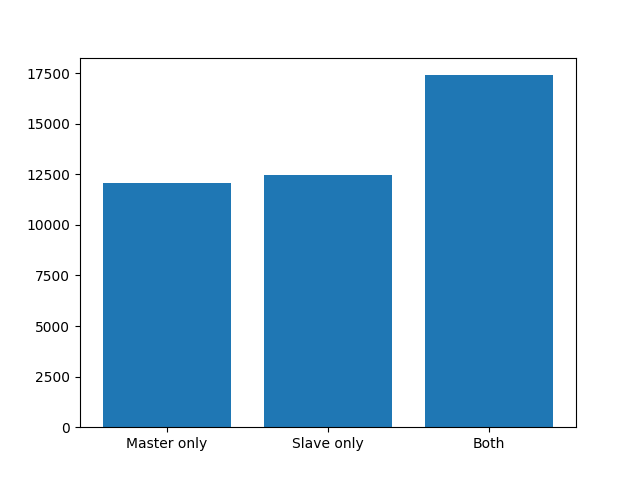
\includegraphics[width=0.8\columnwidth]{domains_vulnerability}
\caption{Domains Vulnerability}
\label{fig:domains_vulnerability}
\end{figure}

To investigate the vulnerability of different types of servers, we repeat our tests targeting different groups of DNS servers. For each vulnerable domain we prepared a list of primary and secondary name servers based on actively queried \texttt{NS} and \texttt{SOA} records. In the first experiment, we sent injects only to primary servers and queried primary and secondary servers right away and after 24 hours. In our second experiment, we targeted the secondary servers uniquely and again queried all the servers right away and after 24 hours. 

The majority of the domains can be attacked using both their primary and secondary servers(Fig. \ref{fig:domains_vulnerability}). However, more than 24,000 domains were vulnerable when attacked using one type of servers. Surprisingly, we discovered a similar amount of domains having vulnerable primary and secondary servers. 

\begin{table}[!htbp]
\centering
\caption{Propagation}
\label{tab:propagation}
\begin{tabular}{@{}lcccc@{}}
\toprule
 & \multicolumn{2}{c}{\textbf{\begin{tabular}[c]{@{}c@{}}Master\end{tabular}}} & \multicolumn{2}{c}{\textbf{\begin{tabular}[c]{@{}c@{}}Slave\end{tabular}}} \\ %\midrule
 & \multicolumn{1}{c}{\textbf{\begin{tabular}[c]{@{}c@{}}0h\end{tabular}}} & \multicolumn{1}{c}{\textbf{\begin{tabular}[c]{@{}c@{}}24h\end{tabular}}}& \multicolumn{1}{c}{\textbf{\begin{tabular}[c]{@{}c@{}}0h\end{tabular}}} & \multicolumn{1}{c}{\textbf{\begin{tabular}[c]{@{}c@{}}24h\end{tabular}}} \\ \midrule
Domains
 & 29479 & 28242 & 29883 & 25268\\ \midrule
Servers
 & 4514 & 4498 & 6526 & 6444\\ \midrule
 Propagation
 & 1643 & 1645 & 15 & 16\\ \bottomrule
\end{tabular}
\end{table}

We then investigate the evolution of the number of affected domains and servers over time (Tab. \ref{tab:propagation}. Querying affected domains directly after sending the inject reveals a similar number of domains for both primary and secondary servers. However, after 24h, the entries injected using secondary servers disappear at a much higher rate than those injected using primary servers. The entries disappear when corresponding, unaffected primary server, propagates the correct configuration to the infected secondary server. 

We also investigate the number of servers affected using both types of injects. Targeting primary servers results in a significantly lower number of affected servers. This is because of a higher number of secondary servers for each affected domains. The number of affected servers remains stable throughout our experiment. 

Finally, we investigate if a vulnerable server is able to infect other servers with an updated configuration. When targeting primary servers, we discovered more than 1,600 secondary servers that downloaded the incorrect zone information. We discovered a significantly lower number of secondary servers pushing changes to the primary one. This is understandable, as if configured correctly, secondary servers are not allowed to update zones. In both cases, the number of affected servers increase slightly over time. 

\subsection{Fingerprinting of vulnerable name servers}
